% 
% Author: Riccardo Orizio (R)
% Date: Thu 24 May 2018
% 
% Description: UCC Poster for Postgrad Review Day on 05/06/2018
%

% Options for format can be included here
\documentclass{tikzposter}
%	\geometry{paperwidth=841mm,paperheight=1205mm}
\geometry{paperwidth=850mm,paperheight=1355mm}

\usepackage[english]{babel}
\usepackage{amsmath}
\usepackage{graphicx}
\usepackage{subcaption}
\usepackage{caption}

% Removing the watermark: still yet to decide if I really want to remove it
%	\tikzposterlatexaffectionproofoff

% Title, Author, Institute
%	\title{Cyber Physical Systems diagnosis: different approaches}
\title{Improving Security and Resilience of Cyber Physical Systems}
\author{Riccardo Orizio, Prof. Gregory Provan}
\institute{University College Cork}
\titlegraphic
{
	
\includegraphics[width=0.13\textwidth]{./Images/logo_sfi.png}
	\hspace{0.2\textwidth}
	
\includegraphics[width=0.13\textwidth]{./Images/logo_ucc.png}
	\hspace{0.2\textwidth}
	
\includegraphics[width=0.13\textwidth]{./Images/logo_lero.png}
}

% Title settings
% Rescaled all text by one factor in comparison to the original settings
\settitle
{
	\centering
	\vbox
	{
		\@titlegraphic \\[\TP@titlegraphictotitledistance]
		\centering
		\color{titlefgcolor}
		{\bfseries \huge \sc \@title \par}
		\vspace*{1em}
		{\LARGE \@author \par}
		\vspace*{1em}
		{\Large \@institute}
	}
}

% Choose Layout
%	\usetheme{Default}
%	\usetheme{Rays}			%	<--
%	\usetheme{Basic}
%	\usetheme{Simple}
\usetheme{Envelope}		%	<--
%	\usetheme{Wave}
%	\usetheme{Board}		%	<--
%	\usetheme{Autumn}
%	\usetheme{Desert}

%	\usecolorpalette
%	\usecolorpalette{Default}
%	\usecolorpalette{BlueGrayOrange}
%	\usecolorpalette{GreenGrayViolet}
%	\usecolorpalette{DPurpleGrayBlue}
%	\usecolorpalette{DBrownBlueOrange}

%	\usecolorstyle
%	\usecolorstyle{Default}
%	\usecolorstyle{Australia}	% <--
\usecolorstyle{Britain}		% <--
%	\usecolorstyle{Sweden}
%	\usecolorstyle{Spain}
%	\usecolorstyle{Russia}
%	\usecolorstyle{Denmark}
%	\usecolorstyle{Germany}

\begin{document}
	% Title block redimensioned due to length of the title
	\maketitle[width=0.9\textwidth]

	% General problem introduction
	\block{General Problem}
	{
		Cyber Physical Systems are systems made of three main parts: physical
		processes, computational resources and communication capabilities.
		These systems can represent many real systems, including complex and
		safety critical ones such as transportation networks, electrical and gas
		distribution, water treatment plants and SCADA systems.
		These critical systems need to operate reliably in all circumstances,
		therefore they need to be able to recover from faulty components
		behaviours as well as from external malicious attacks.

		Our goal is to improve the resiliency of the system, starting from the
		current most used model based approach and expanding to new techniques.

		%	Diagnosis has always been a very interesting and difficult subject to
		%	deal with: the need of knowing the reasons behind malfunctions in all
		%	kind of systems pushed people to study this topic.
		%	Malicious attacks have always been a threat for systems, but with the
		%	growth of Internet, they increased in number and in effectivness.
		%	This is the main reason why diagnosis needs new methods to deal with all
		%	kind of anomalies, either genuine or not.

		%	With the growth of Internet, malicious attacks are one more reason to 
		%	genuine malfunctions are not the only
		%	Genuine malfunctions of components part of the system is not the only
		%	reason why diagnosis exists.
		%	Now more than ever, due to the growth of Internet and the need to
		%	connect all systems to it, the need to prevent malicious attacks that
		%	can be injected to the systems.

		%	Here we present different approaches to work on CPS, in particular our
		%	goals are: \textbf{detection} of unusual behaviour,
		%	\textbf{identification} of the component causing the anomaly and
		%	\textbf{distinction} of the cause of the anomaly, either fault or
		%	attack.

		%	\begin{itemize}
		%		\item[-]{Detection of unusual behaviour;}
		%		\item[-]{Identification of the component causing the anomaly;}
		%		\item[-]{Distinguishing the cause of such anomaly: fault or attack.}
		%	\end{itemize}
	}

	\block{Distinguishing Faults from Attacks}
	{
		\begin{minipage}[t]{\linewidth}
			\centering
			\vspace{-100mm}
			\begin{minipage}[t]{0.45\textwidth}
				To improve the system security and resiliency we need to:

				\vspace{5mm}

				\begin{itemize}
					\item[-]{\textbf{Detect} the unusual behaviour;}
					\item[-]{\textbf{Identify} the component causing the anomaly;}
					\item[-]{\textbf{Distinguish} the cause of the anomaly, either fault or attack.}
				\end{itemize}
				In order to achieve our purpose, we introduced two components to the
				system:
				
				\vspace{5mm}

				\textit{\textbf{Sensor filter}}: estimates the state of
				components knowing the sensors data.

				\textit{\textbf{Actuator filter}}: helps distinguishing the
				anomaly by delaying the current control signal of one step.

			\end{minipage}
			%%
			\vspace{50mm}
			%%
			\begin{minipage}[c]{0.43\textwidth}
				\centering
				\vspace{100mm}
				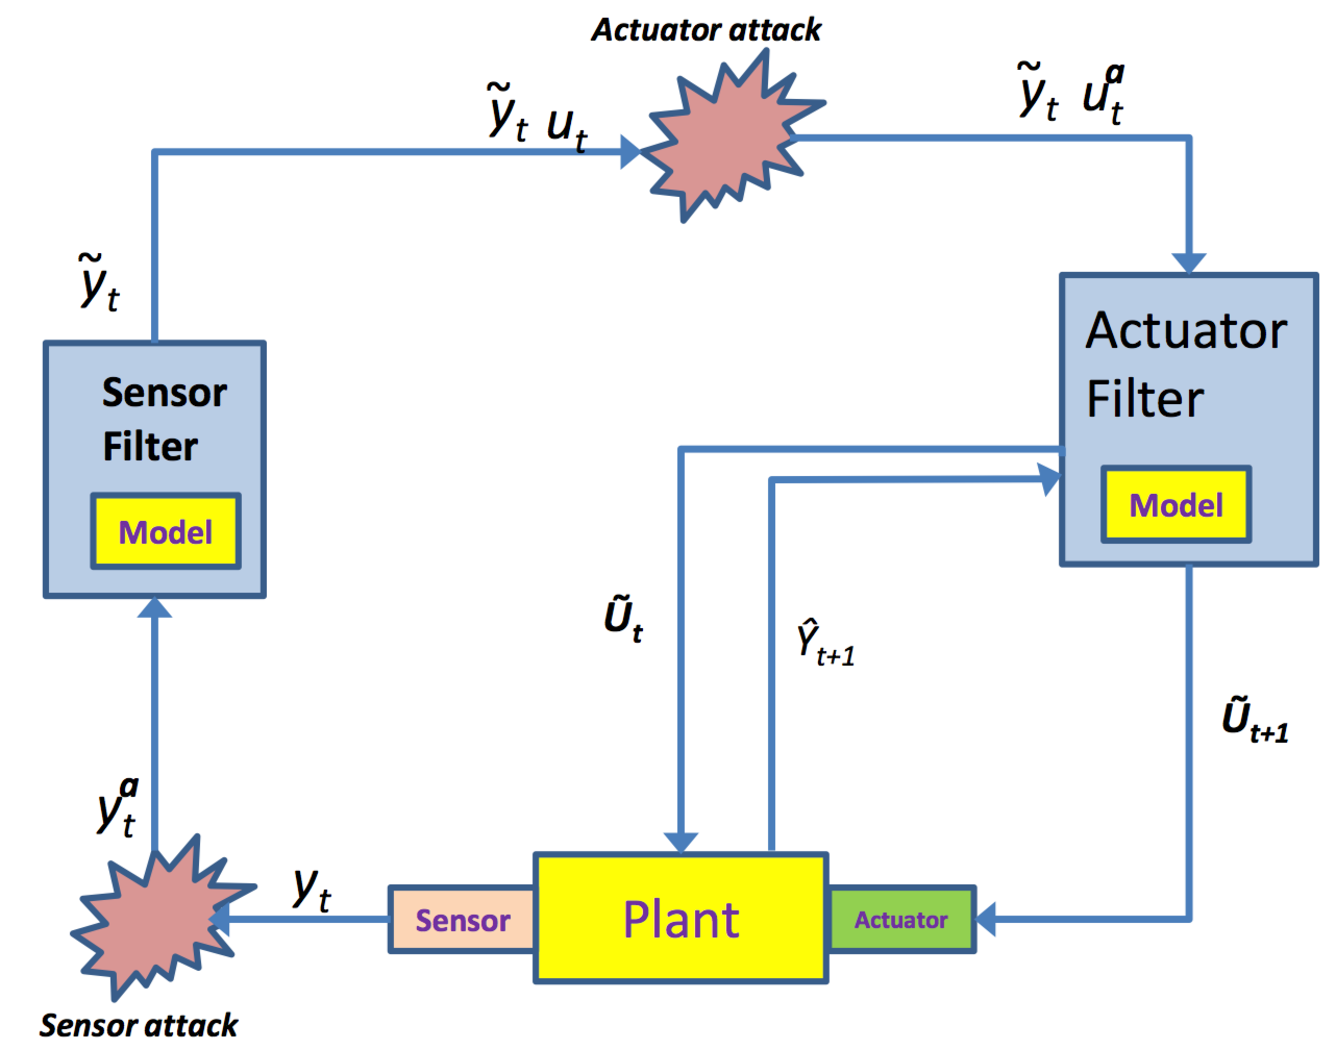
\includegraphics[height=15cm]{./Images/system_architecture.pdf}
			\end{minipage}

		\end{minipage}
%
		%	The next step is to try to disinguish genuine malfunctions from
		%	malicious attacks.
		%	A new idea that we proposed is to use the system itself to our
		%	advantage: an attack to data readings of the system does not affect the
		%	internal state of the system and therefore its following data readings
		%	should not be different from what we are expecting.
		%	The idea is to wait one step before sending the control signal to the
		%	system and try to understand if the anomaly is due to an attack or a
		%	real fault.
		%	This approach together with the algebraic diagnoser seem to be
		%	effective.
%
		%	\vspace{5mm}
%
		\begin{minipage}[t]{\linewidth}
			\centering
			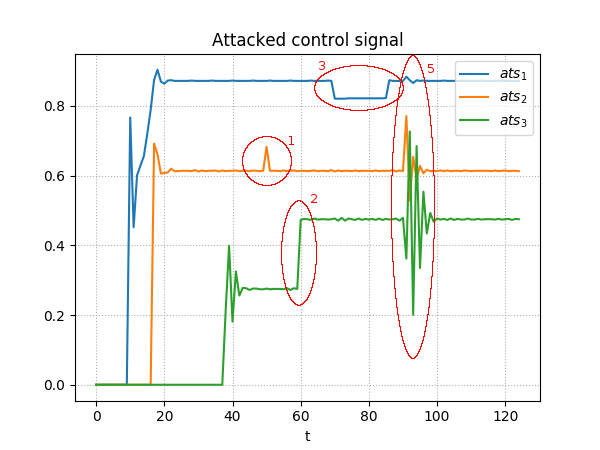
\includegraphics[height=10cm]{./Images/attacked_signal_improved.png}
			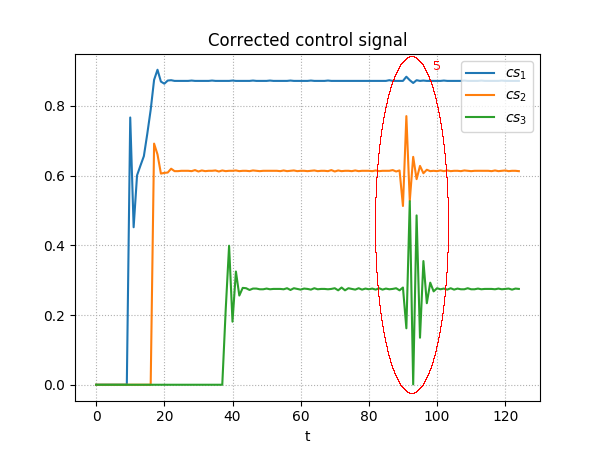
\includegraphics[height=10cm]{./Images/control_signal_improved.png}
			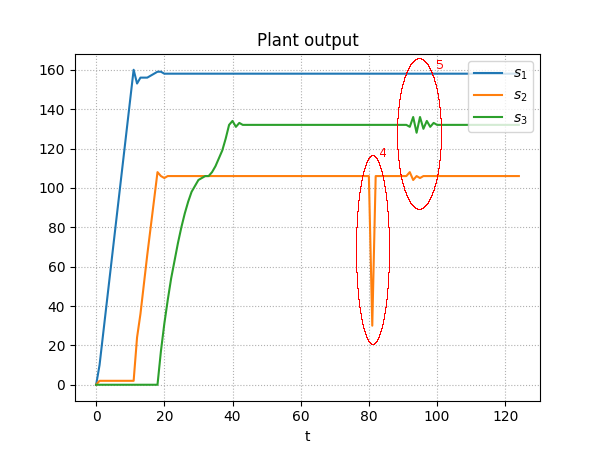
\includegraphics[height=10cm]{./Images/sensors_improved.png}
		\end{minipage}
	}

	\begin{columns}
		\column{0.5}
		{
			\block{Model Based Approach}
			{
				A system can operate in different modes (e.g. some drone
				operating modes can be taking-off, landing, wandering,
				surface-mapping, etc...).
				Each mode can be identified through a mathematical model,
				knowing its current internal state $x_i$:

				\vspace{10mm}

				$$
				\text{Modes}: 
				\begin{cases}
						\ y_{m_1} = f_1(x_i)	\\
						\ y_{m_2} = f_2(x_i)	\\
						\qquad ...				\\
						\ y_{m_n} = f_n(x_i)	\\
				\end{cases}
				$$

				\vspace{25mm}

				\textit{\textbf{Forward inference}}: compute the mode behaviour
				$y_j = f_j(x_i)$

				\vspace{10mm}

				\textit{\textbf{Inverse inference}}: find the internal state
				that led to the current behaviour $x_i = f^{-1}_{j}(y_j)$
		
				The inverse inference is a difficult procedure to perform when
				$f_j$ is linear, in most CPS these modes are non-linear.

				\vspace{10mm}
		
				\textit{\textbf{Diagnosis}}: inverse inference including faulty
				modes in the set of modes.
			}
		}

		\column{0.5}
		{
			\block{Data Driven Algebraic approach}
			{
				\begin{itemize}
					\item[-]{System's sensors data and its derivatives analysis
						(derivatives studied up to third order);}

					\item[-]{Looking for unusual \textit{peaks} in the data
						behaviour and their neighborhood.}
				\end{itemize}
				%	Data analysis of the system's sensors observed data looking for
				%	easily recognizable characteristics.
				%	The analysis studies the data and all its derivatives up to the
				%	third order.
				%	Specifically we look for unusual peaks and how the behaviour
				%	changes around them to identify the class of anomaly that has
				%	happened.

				%	The operations performed during the analysis are computationally
				%	not intensive, basic operations and comparisons, and increase
				%	linearly in number with the data set.

				\vspace{15mm}

				\begin{center}
					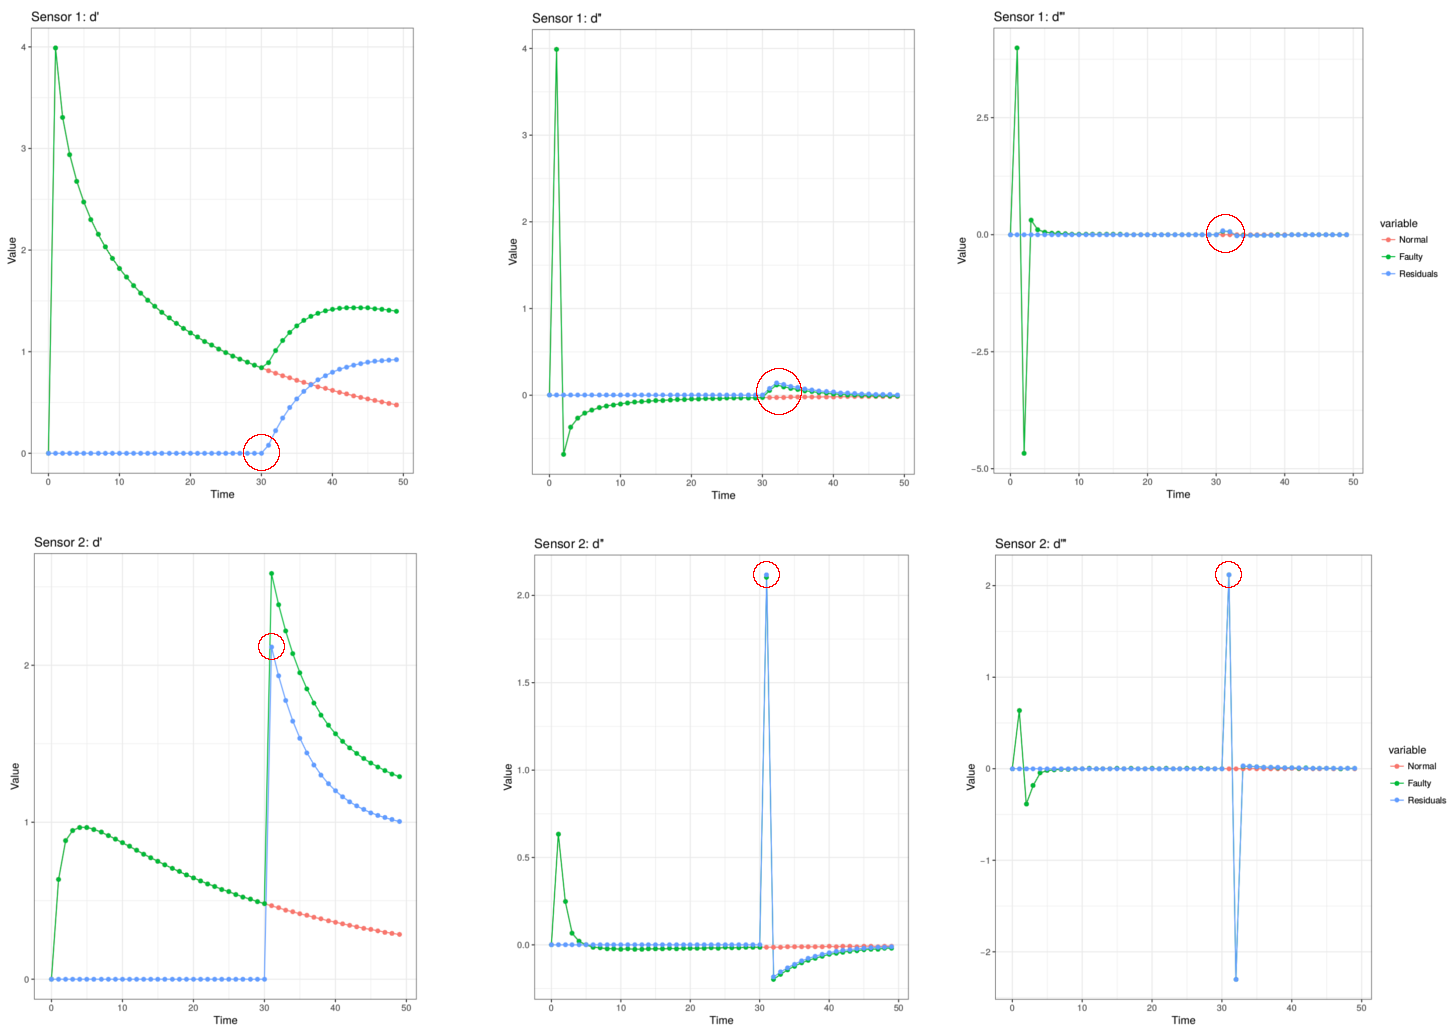
\includegraphics[height=20cm]{./Images/attack_peak_circled.png}
					%	\captionof{figure}{Example of derivatives data being
					%	studied. Sensor 2 is under attack (clear peak in all
					%	derivatives); sensor 1 shows the reaction of the system due
					%	to the anomaly (smoother peak).}
				\end{center}

			}
		}
	\end{columns}

	\block{Model Based or Algebraic approach?}
	{
		We compared the two approaches on the same set of experiments, finding:
		\begin{itemize}
			\item[-]{Algebraic approach seems better;}
			\item[-]{Masked multi-anomalies and synergistic behaviours seem to
				be easier to detect with the algebraic approach than it is with
				the model based one.}
		\end{itemize}
		%	We compared the two approaches on the classical three tanks system and
		%	the results showed that, even if the algebraic diagnoser does not have
		%	all the features that we want, it outperforms the model based approach.
		%	Masked multi-anomalies and synergistic behaviours seem to be easier to
		%	detect with the algebraic approach than it is with the model based one.

		\vspace{5mm}

		\begin{minipage}[t]{0.40\textwidth}
			\centering
			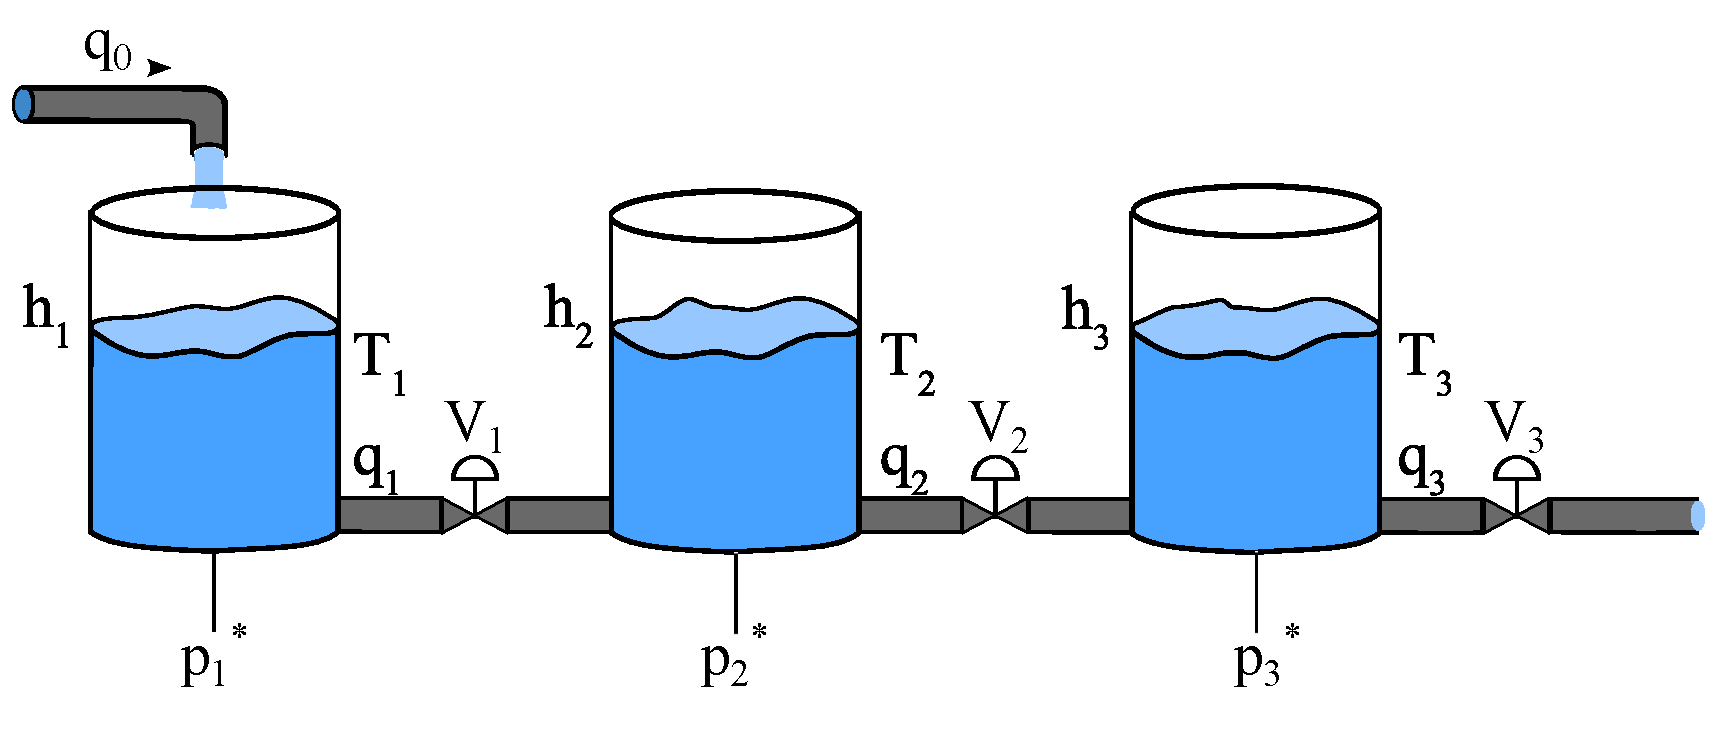
\includegraphics[height=10cm]{./Images/3-tanks.pdf}
			%	\captionof{figure}{Three tanks system.}
		\end{minipage}
		%%
		%	\vspace{15mm}
		%%
		\begin{minipage}[t]{0.43\textwidth}
			\centering
			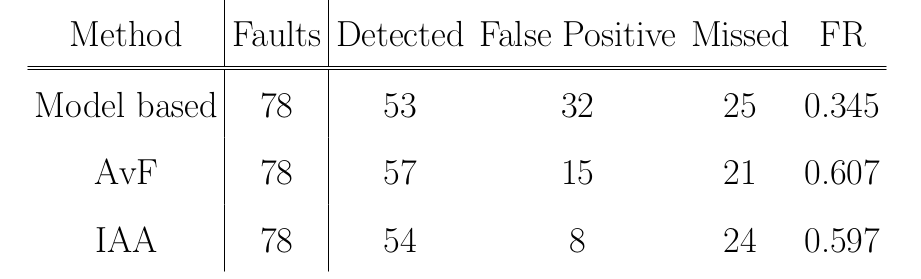
\includegraphics[height=9cm]{./Images/comparison_results.png}
			%	\captionof{figure}{Approaches comparison results on multi anomalies results.}
			%	%	\begin{table}[h]
			%		\centering
			%		\renewcommand{\arraystretch}{1.5}
			%		\begin{tabular}{ c | c | ccc c }
			%			Method & Faults & Detected & False Positive & Missed & FR \\
			%			\hline
			%			\hline
			%			Model based	&	78	&	53	&	32	&	25	&	0.345	\\
			%			AvF		&	78	&	57	&	15	&	21	&	0.607	\\
			%			IAA		&	78	&	54	&	8	&	24	&	0.597	\\
			%		\end{tabular}
			%		%	\captionsetup{width=0.9\linewidth}
			%		\captionof{table}{Multi-faults results}
			%		\label{tab:results_mixed}
			%	%	\end{table}
		\end{minipage}
	}

	\begin{columns}
		\column{0.5}
		{
			\block{Papers contribution}
			{
				\begin{itemize}
					\item[-]{\textit{Physics-Based Methods for Distinguishing Attacks from Faults}, CENICS 2017}
					\item[-]{\textit{Comparing Physics-Based Methods for Distinguishing Attacks from Faults}, DX'18}
					\item[-]{\textit{Physics-Based Methods for Responding to Attacks and Faults}, WIP}
				\end{itemize}
			}
		}
		%%
		%	\hspace{15mm}
		%%
		\column{0.5}
		{
			\block{Future}
			{
				\begin{itemize}
					\item[-]{Integrate machine learning techniques to make the
						procedure self-aware to different behaviours and their
						classification;}
					\item[-]{Signal Temporal Logic approach for diagnosis;}
					\item[-]{Extension to other real-world applications (e.g. FCU).}
				\end{itemize}
			}
		}
	\end{columns}

\end{document}

